%! TeX root = ../Parte2.tex

\section{Blocco dei tracker}

\begin{myframe}{Blocco tracker pubblicitari}
  Spesso gli annunci pubblicitari ci tracciano: sanno che pagine visitiamo\\ e quanto ci soffermiamo in determinati punti.

  \medskip\pause
  uBlock Origin blocca gli annunci pubblicitari sulle pagine web\\ e molti altri elementi traccianti.
\end{myframe}


\begin{myframe}{Blocco tracker su Firefox}
  Firefox fornisce di default molte impostazioni per il blocco degli elementi traccianti.

  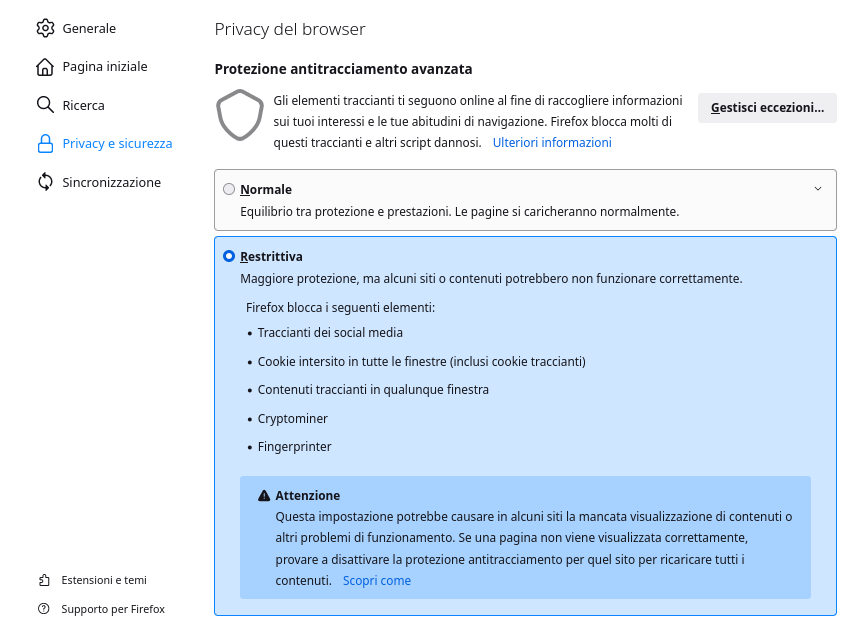
\includegraphics[width=.7\textwidth]{img/firefox_tracker}
\end{myframe}


\begin{myframe}{Firefox containers}
  Inoltre attivando i containers si possono creare dei \textbf{profili} da usare per \textbf{siti diversi}.

  Così da non condividere i cookie traccianti, ma anche permettendo l'uso di account diversi senza sloggarsi.

  \smallskip
  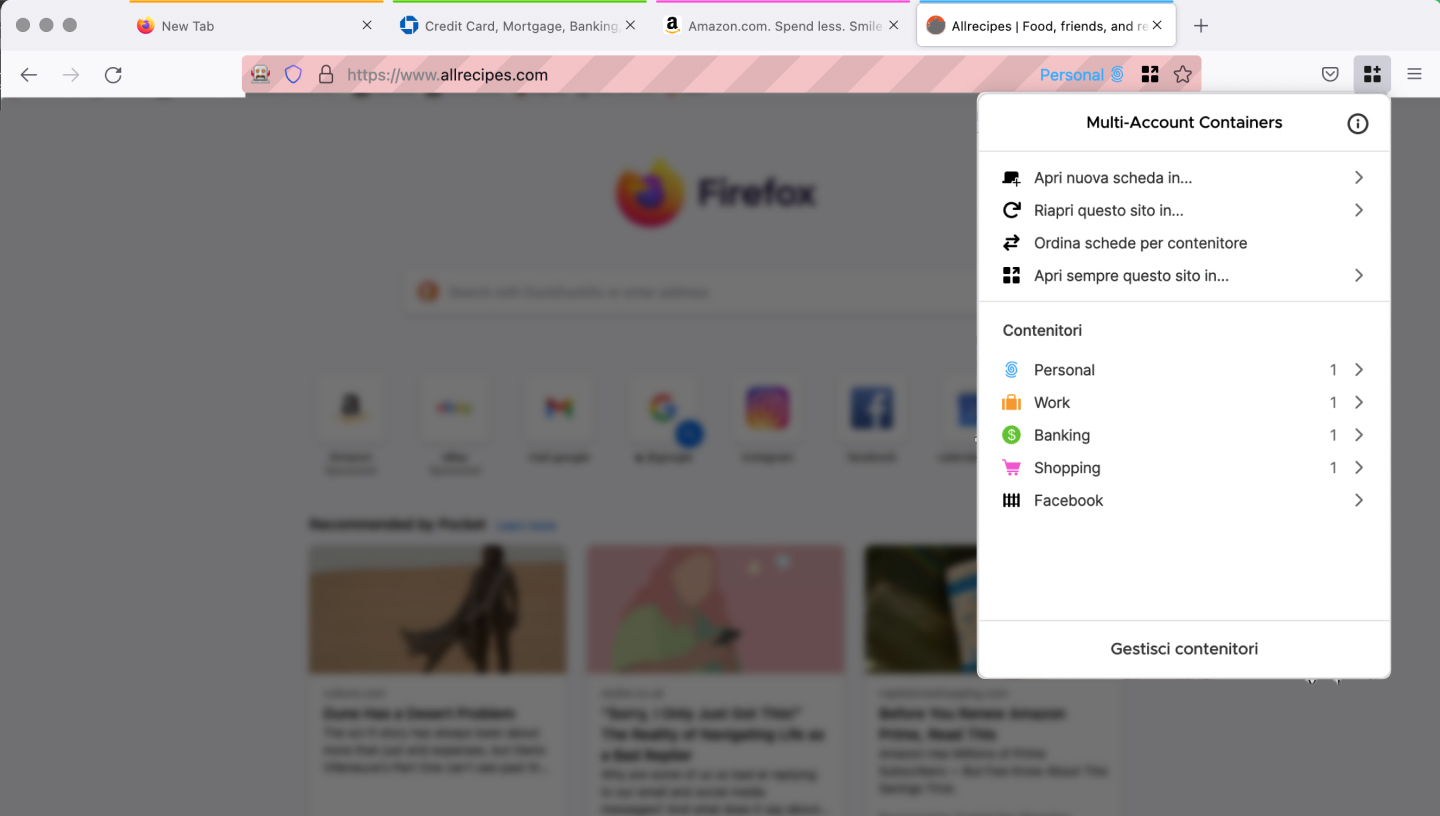
\includegraphics[width=.7\textwidth]{img/firefox_containers}
\end{myframe}

\begin{myframe}{Facebook container}
  Esiste un container particolare chiamato ``Facebook container'' che reindirizza in automatico tutte le pagine di Meta a lui.

  Protegge anche dai pulsanti ``Mi piace'' presenti nelle pagine web disabilitandoli.

  \smallskip
  
\includegraphics[width=.8\textwidth]{img/facebook_container}
\end{myframe}

\begin{myframe}{Altre estensioni}
  \begin{description}
    \item[HTTPS everywhere / Firefox HTTPS-only] Reindirizza alla versione https dei siti se disponibile;
    \item[Decentraleyes] Elimina chiamate a CDN;
    \item[Privacy badger] Blocca molti tracker.
  \end{description}
\end{myframe}

\begin{myframe}{DNS}
  Un DNS traduce un url (\texttt{duckduckgo.com}) in un indirizzo ip (\texttt{40.114.177.156}).

  \medskip\pause
  Il server DNS sa che siti visitiamo.

  \medskip\pause
  Esistono \textbf{DNS non traccianti} che possiamo usare.

  Ad esempio AdGuard DNS oltre a non tracciarci \textbf{blocca anche alcuni tracker}. Se lo impostiamo nel router protegge anche altri dispositivi (come smart TV).

  \medskip\pause
  DNS over Https (DoH) o TLS (DoT) permettono di criptare le chiamate al DNS che altrimenti sarebbero in chiaro.
\end{myframe}

